\documentclass[12pt,a4paper]{article}  
%\usepackage{fullpage} %for minimal marginal  
\usepackage[utf8]{inputenc}    %encoding

\usepackage[english]{babel} %English sections
\usepackage{graphicx}    %For the possibility of pictures
\usepackage{amssymb, amsmath} %for American Math. society symbols and environments etc.
\usepackage{supertabular} % For tables that are larger than one page
\usepackage{longtable} %for longer tables 
\usepackage{multirow} %If one want to have the text in several rows
\usepackage{tabularx} %Tables with dynamic cell-sizes
\usepackage{multicol} %Nödvändigt om man vill ha flera kolumner

%Figure captions must be at the bottom
\usepackage{floatrow}
\floatsetup[figure]{capposition=bottom}
\floatsetup[table]{capposition=top}

%This is so that I dont need to have figure-captions that are wider than the text (really ugly)
\usepackage{caption}
\usepackage{lipsum}


%% Images with a different path to the parent latex file can
%% be accessed with the `import' package (which may need to be
%% installed) using usepackage import
\usepackage{import}

%I want footnotes with Roman letters...
\renewcommand{\thefootnote}{\roman{footnote}}

%BibLaTeX grejer...
%Explanation:
%style sets the format of the reference list at the end of the report
%citestyle sets the format of the cites
\usepackage[backend=bibtex,style=chem-acs,citestyle=chem-acs]{biblatex}

%\bibliographystyle{unsrt}
\bibliography{references}


%XX YET TO COME

%%%%%%%%%%%Brja deklarationen av bilder i multicols%%%%%%%%%%%%%%%%%%%%%%%%%%%%
\newcounter{myFCounter}[section]
\newcommand{\myFigure}[3]{%
    \begin{center}\begin{minipage}[t]{\columnwidth}%
    \begin{center}\refstepcounter{myFCounter}\vspace{1ex}%
    \includegraphics[width=#1\columnwidth,keepaspectratio]{#2}\ \\%
    \sc Figure \thesection .\arabic{myFCounter}:\ \rm #3 
    \vspace{1ex}\end{center}%
    \end{minipage}\end{center}}

%%%%%%%%%%%%%%%%%%%%%%%%%%%%%%%%%%%%%%%%%%%%%%%%%%%%%%%%%%%

\author{Sara Kjellberg}
\title{Surface functionalization of H-terminated diamond with NH and NH$_2$ on the (1 0 0), (1 1 0) and (1 1 1) surface planes using Density Functional Theory.}

\begin{document}
\begin{titlepage}
	\centering
	
\includegraphics[width=0.15\textwidth]{pictures/uulog.png}\par\vspace{1cm}
	{\scshape\LARGE Uppsala University \par}
	\vspace{1cm}
	{\scshape\Large Bachelor project, 15hp\par}
	\vspace{1.5cm}
	{\huge\bfseries Surface functionalization of H-terminated diamond with NH and NH$_2$ on the (1 0 0), (1 1 0) and (1 1 1) surface planes using Density Functional Theory\par}
	\vspace{2cm}
	{\Large\itshape Sara Kjellberg\par}
	\vfill
	Supervised by\par
	Prof.~Karin \textsc{Larsson}

	\vfill

% Bottom of the page
	{\large \today\par}
\end{titlepage}
%\maketitle
%\begin{figure}[t] \captionsetup{width=.8\linewidth}
%
\includegraphics[width=2cm]{pictures/uulog.png}
%\end{figure}
%\hrulefill %skriv ut en linje
\abstract{The adsorption energy of aminated diamond surfaces on the (1 1 1), (1 1 0) and (1 0 0) diamond surfaces have been calculated with density functional theory (DFT). The resulting values show that bridging is favoured before on-top nitrogen at low coverage for all the low index planes. The trend is even more pronounced as the coverage increases, most likely due to sterical hindrance. As expected, the imidogen (NH) and amidogen (NH$_2$)  groups are bonded to the surface planes in the order (1 0 0)$>$(1 1 1)$>$(1 1 0) as decrease in energy is the highest on the (1 0 0) plane and lowest on the (1 010) plane. The effect of sterical hindrance is largest at the (1 1 0) surface while the (1 0 0) surface is almost unaffected by neighbouring functional groups. Also, double bonded on-top imidogen (NH) is the least stable group at the (1 0 0) surface at low coverage while it is almost as stable as bridging NH when having a full mono-layer. Moreover, on-top imidogen (NH) was highly distorted and forced a change in surface geometry}

\newpage
%\hrulefill %skriv ut en linje
\tableofcontents
\newpage

\section{Goal}
The goal of this study was firstly to find out which one of amidogen (NH$_2$) and imidogen (NH, on-top or bridge) is theoretically most strongly bonded to a diamond surface. Secondly to find out whether NH$_2$ or NH (on-top or bridge) is theoretically best attached to a (1 0 0), (1 1 0) or (1 1 1) oriented diamond surface.

\section{Introduction}
\subsection{Background}
%\textbf{I may use this section if it is allowed to use a summary of other articles. }
Diamond, and in particular nanodiamond, has become a promising candidate for several fields of application. One of those applications is to use it in medical and biological sciences as it possess biocompatibility  as well as good chemical and electrical properties. It also has a large electro-potential window, which may be further enhanced or inhibited by modifying the surface. Furthermore, even though diamonds show good physical/chemical stability, the surfaces are still easily modified or functionalized by photochemical reactions \cite{c.e.nebel2007}.
%(\textit{Review. Diamond and biology } C.E. Nebel  \textit{et. al.}) 

%\paragraph*{}
%Analytica Chimica Acta 573-574 (2006), 3-8
%Adding amidogen and imide to surfaces changes makes the diamond surface more sensitive to pH, wich might be medical use as some diseases makes the pH lower or higher than normal. 
To use diamond for medical purposes such as the growing of bones, proteins and DNA must first be successfully attached to the diamond surface. One way to enhance the attachment of these types of molecules is functionalizing surfaces with various biologically common functional groups before trying to bind the specific molecule to the surface. Amine-based groups in particular may be a good step on the way to so this since both imidogen (NH-) and amidogen (NH$_2$) are part of many well known biochemical and organical reactions. This has already been done as preliminary step in binding DNA to a diamond surface. Aminating the surface by UV-radiation will also make the surface pH sensitive depending on the amount of UV-radiation. Furthermore, amidogen (NH$_2$, on-top) groups produced by long-term UV-radiation have proven to be stable under exposure to air. \cite{kwang-soup.song2006}. It has also been reported that diamond has high stability and sensibility as well as compatibility with microelectronic processing technology. All of these properties also make diamond a promising candidate for  biological integration of microelectronics as well as biological modification \cite{yangwenshaw2002}. 

%In applications such as mentioned, a thin film is often requered rather than a large bulk. The main method of creating thin films in general is Chemical Vapour Deposition (CVD)  \cite{inorganicchemistrybook}. 

There are also several well established ways to produce diamond in industrial and laboratory settings aside from CVD (Chemical Vapor Deposition). Naturally, the surface chemistry will vary depending on chosen method. Specifically, nano-diamonds can for example be produced using shock waves (so called shock-wave diamond) or explosives (detonation diamond) on carbon materials. The surface of shock-wave diamond is graphitized and detonation diamond is covered with various oxygen containing groups. The surface of detonation diamond have been successfully homogenised using oxidative (yielding for example mostly keto- and carboxyl-groups) or reductive methods with the latter yielding, for example, an H-terminated or OH-terminated surface. CVD-diamond will, generally, yield an H-terminated surface without further cleaning or homogenisation.\cite{ankekrueger2007} Also, several studies have already been made concerning low-index planes of diamonds, mostly practical work, but also some purely computational studies. Some of those cover the adsorption of amines on diamond.  One of these are a relatively early study that regarded the full coverage (mono-layer) of NH$_2$ on the (1 1 1), (1 1 0) and (1 0 0) planes of diamond surfaces. They used MM (Molecular Mechanics). The results showed that full coverage meant great distortion of the structure at the (1 1 0) and (1 1 1) cleavage of the diamond surface. Although the report did not report either enthalpies or adsorption energies, this may indicate that full coverage is unlikely. The (1 0 0) surface did not show any significant distortion. \cite{johnb.miller2001}

Another, slightly more recent study has been done regarding adsorption of NH$_2$ on a reconstructed (1 0 0)-diamond surface using DFT (Density Functinal Theory) with the GGA (General Gradient Approximation) approximation. The resulting energies, while comparing a structure with two nearby NH$_2$ groups with one with hydrogen instead, showed that the energy levels were lower in the latter case. It is hence unlikely that two amino-groups will form in two nearby reaction sites at the reconstructed (1 0 0) diamond surface. \cite{yan.dong2010}

Amidogen (NH) and Amine (NH$_2$) adsorption has also been found to be energetically favoured around room temperature on the (1 0 0), (1 1 0), and (1 1 1) planes of nanodiamond using density functional tight binding simulations.  \cite{lin.lai2011}

\section{Theory}
\subsection{Surfaces of diamond}
\subsubsection{General surface theory}
The reactivity of a crystal surface is known to be dependent of the surface structure and morphology, which do not only depend on the crystal lattice, but also the orientation of the intersection in relation to the crystal lattice. Both coordination numbers and numbers of possible reaction sites differ depending on plane (orientation of the intersection) and surface morphology. The specific plane is formally described using miller indexes where the numbers represent the intersection through the three mayor crystallographic axes of the lattice. The three most simple surface planes are (1 1 1), (1 1 0) and (1 0 0) but it is possible to use higher indexes. The (1 1 1), (1 1 0) and (1 0 0) planes are demonstrated in figure \ref{millerindex}. Naturally, properties that generally leads to larger surface energy such as large surface areas and low coordination numbers on surface atoms generally means a higher reactivity and a stronger binding of an adsorbate. Another property that affect surface energy, and thus its reactivity, is how close-packed the surface atoms are. The direction of free bonds at the radical surface also plays a role in how well an adsorbate can be bonded to the surface \cites{surfaces, BAHC}. 

\begin{figure} \captionsetup{width=.8\linewidth}
\caption{A description of the  (1 0 0), (1 1 1) and (1 1 0) planes. This picture was picked from an online glossary \cite{millerindex}, but the same information can be found in any book pertaining basic solid state chemistry} \label{millerindex}
%\input{pictures/products.pdf_tex}
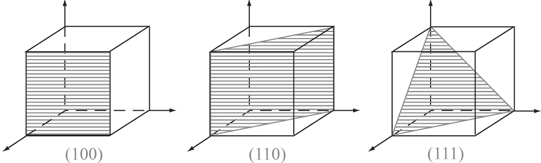
\includegraphics[width=.8\linewidth]{pictures/millerindex.png}
\end{figure}

\subsubsection{Structure of the low index surfaces of diamond}
For simplicity, this study only explores the adsorption of ammonia on diamond at the three low-index surfaces (1 1 1), (1 1 0) and (1 0 0). The overall structure of diamond is a derivative of the zinkblendestructure where all atoms are the same (se figure \ref{diamond_general}). In other words, all carbon atoms in the bulk have the coordination number 4 meaning sp$^3$-hybridisation and a tetrahedral symmetry around the atoms  (se figure \ref{diamond_general}). A closer look at the three planes show that the surface atoms has the same coordination number, which is three, but the rest is different. The (1 0 0) plane does not keep perfect tetrahedral symmetry around the carbon atoms at the surface and are less close-packed than the other two planes studied and is therefore expected to have the largest surface energy.  One might even speculate that it is possible for a bond to break between two neighbouring surface atoms, creating lower coordination numbers. In comparison, the (1 1 0) and (1 1 1) planes do keep the tetrahedral symmetry around the carbon atoms. One can also see that while the surface of the (1 1 1) plane seem more close-packed than the (1 1 0), the free bonds of the latter is actually closer to each other in the latter case. A schematic illustration displaying the free bonds (refererred to as dangling bonds) of the three planes is shown in figure  \ref{dangling_bonds}. 

\begin{figure} \captionsetup{width=.8\linewidth} \caption{The general lattice of diamond. This picture was generated on a free, online resource center, but the same information can be obtained in many ways and the diamond structure as well as the that of zinkblende are both to be considered general nowledge.} \label{diamond_general}
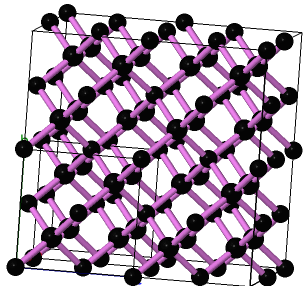
\includegraphics[width=.8\linewidth]{pictures/diamond_general.png}
\end{figure} 

\begin{figure} \captionsetup{width=.5\linewidth} \caption{Schematic illustration displaing the dangling bonds of the (1 1 1), (1 1 0) and (1 0 0) plane from the side (top) and from above (bottom).} \label{dangling_bonds}
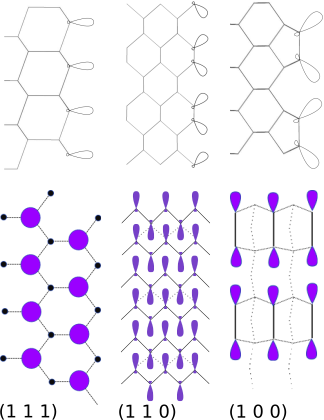
\includegraphics[width=.5\linewidth]{pictures/dangling_bonds.png}
\end{figure} 

\subsection{General computional theory}
Molecular modelling is a good way to get a further understanding of the workings of chemical systems and molecules.  Not only can one study reactions that are either strictly theoretical or either to dangerous or hard to study in a practical experiments. Environments can easily be strictly defined (thus isolating problems and trend factors from each other) from other factors) and properties that would otherwise be very hard, impossible or very expensive might be studied. There is however, no perfect model simulating an exact replica of the real world, which gives all the answers. It is, specifically, impossible to get an exact and true electron configuration.

There are hence several different approaches and methods developed for modelling chemical systems, each using their own approximations that have their own pros and cons. Those use quantum mechanics, molecular mechanics  or a statistical approach. Quantum mechanical methods are, in essence, solving the problem by approximate solutions of the Shcrödinger equation.  Molecular mechanics uses classical mechanics and replace the electrons with a fixed force field that represent  them. Molecular mechanics might generate properties such as temperature dependence, different kinetical properties and even information about systems that are not in equilibrium.  The statistical approach uses the inherent statistical properties that exist within all systems and will therefore only give information about systems in equilibrium, which those methods are very good at. Both molecular mechanics and methods that use statistics are cheap in computational time and requirement, so very large systems can be simulated at a short time. They do not, however, give any information about electron configuration (which is what this study wanted) \cite{computionalprimer}. Hence the quantum mechanical approach had to be used here.

\subsection{Quantum mechanical methods}
\subsubsection{General}
\paragraph*{}
As mentioned earlier, quantum mechanical methods calculates the total energy of a system by 'solving' the Schrödinger equation with the help of various approximations. Those approximations are needed as it is very hard to successfully calculate all interactions between two or more particles. There are therefore not one, but several different approaches for that, and the area is still under development. 

The Schrödinger equation in its most basic form is stated below (see equation \ref{shrodinger1}). H is an operator which operates on a  mathematical function, $\Psi$ is the wave-function and E the energy of the system. $\Psi$ is actually a set of functions with each specific function $\Psi_i$ corresponding to an allowed E$_i$. The functioanal  of the Schrödinger equation (H) is what is referred to the Hamiltonian. 
The Hamiltonian is composed of two parts, the part that comes from the kinetic energy of the system (\^{T}) and the external potential energy of the system (\^{S}). Wave-functions that satisfy the Schrödinger equation are normally called orbitals, which will be used  henceforth. 

\begin{equation} \label{shrodinger1}
H \Psi = ( \hat{T} + \hat{S}) \Psi = E \Psi
\end{equation}
This is a many-body problem and therefore not solvable (one can not get an exact replica of reality), the computational cost will also increase rapidly as the size of the core and number of electrons increase. Therefore, the Born-Oppenheimer approximation will be used from know on in the text.

\paragraph{Explanation: The Born-Oppenheimer approximation:}
The BO-approximation states that the mass of the nuclei are so much larger than that of the electrons that the mass of the electrons is negligible and can be approximated to a fixed field while studying the nuclei. It also states that the movements of the nuclei are so small compared to that of the electrons that the core can be described as fixed points while studying the electrons. In this study, the electrons are studied, so the nuclei will be fixed. 

\paragraph*{}
 The orbitals are not known for poly-electron atoms and molecules, hence the use of approximate orbitals. As it is, when implementing orbitals in a model,  a starting set of wave-functions that satisfy equation \ref{shrodinger1} are used leading to a starting energy. The wave-functions are themselves a linear combination of so called basis functions that are picked from a set of pre-defined functions. The total set of basis functions used in a calculation is referred to the basis set of the calculation. 

\paragraph{Explanation: A basis set} is a set of predefined functions that are used to describe the wave-functions of the system that is being studied. Each wave-function is a linear combination of basis functions. \cite{burke} A plane-wave basis set is a set uses plane wave-functions.

\paragraph{Explanation: A plane wave-function}
A plane wave-function  is a wave-function that is a whole plane rather than a single line. Those can be described using a wave-function and a vector that shows the direction of the plane wave-function. Specific 3-D surfaces can be obtained by combining several non-parallel plane-waves. 

\subsubsection{Plane wave basis sets and cut-off energy}
Plane wave basis functions are, as the name implies, a set of basis functions that uses plane waves instead of ordinary waves. In principle, to get a perfect result, an infinite number of plane waves are needed. Naturally, the accuracy of the result increases while using more functions. That does not prevent good results as one apply Bloch's theorem as well as truncate by only including the most important plane-waves. It has been found that the plane-waves with the smallest kinetic energy is most important. That means that only the plane-waves with a kinetic energy that is below a pre-specified value, the so called cut-off-energy, is needed to be included. 

\paragraph*{}
There is, generally, necessary to use more basis functions than those needed to just describe the electrons surrounding the lone atoms. Naturally, a large basis set both increases the accuracy of the calculation as well as creating a great increase in computational requirement.  There are also different methods to get the energy by solving and optimizing the equation \cite{computionalprimer}.

There are both several basis set and methods to chose from, and the purpose of this study was not to write a book about quantum chemical methods, so no more descriptions of all combinations that were not used will follow.

\subsection{Density Functional Theory (DFT)}
The general concept behind DFT is to treat the electron as an inhomogeneous gas of electrons rather than discreet orbitals. That is, the electron density is calculated for the system as opposed to each electron on their own. DFT is therefore not just another way of solving the Schrodinger equation. \cite{burke} This is a good approach, as Kohn and Hohenberg proved with a simple contradiction  in the year 1964 that the energy of a system is uniquely defined by its electron density and vice versa.  That means that the potential, \^{S} in equation \ref{shrodinger1} can be replaced with a density. The methods for this where developed a year later by Kohn and Sham. The final expression for the energy of an interacting gas in a static potential $v(r)$ and electron density ($n(r)$) that was presented in that report is shown in equation \ref{Kohn_hohenberg}. $G(n)$ is a universal functional of the density.   

\begin{equation} \label{Kohn_hohenberg}
E = G(n) + \int v(r) n(r) dr + \frac{1}{2} \iint (\frac{n(r) n(r')}{|r-r'|})dr dr'
\end{equation}

As an approximation of $G(n)$, Kohn and Sham define the universal functional ($G(n)$) as the sum of the kinetic energy,$T_s(n)$ and the major parts of the effects of the exchange and the correlation energy that stems from the electron-electron and core-electron interaction, $E_{xe}(n)$ (see equation \ref{(G(n)}).
\begin{equation} \label{(G(n)}
G(n) \equiv T_s(n) + E_{xc}(n)
\end{equation}


The hard part of equation \ref{(G(n)} is the correlation energy which can be approximated easily if the electron density does not vary much. Then the correlation energy can be calculated simply as if each electron is in a homogeneous gas of electrons. (equation \ref{homogenous_gas}, $\epsilon_{xc}$ is the correlation and exchange energy per electron in a homogeneous gas with density n). This approach is referred to as the Local Density Approximation (LDA).

\begin{equation} \label{homogenous_gas}
E_{xe}[n] = \int n(r)\epsilon_{xc} n(r) dr 
\end{equation}

Equation \ref{homogenous_gas} do not work well when the density is expected to vary so other solutions or further approximations for the correlation and exchange energy is needed. The solution that Kohn and Sham suggested were the Local Density Approximation (LDA) that can be extended to the General Gradient Approximation (GGA).
\cite{Kohn_and_Hohenberg64}\cite{Kohn_and_Sham65}

\paragraph{Explanation: A functional} is a real valued function on a vector space (usually of functions). The meaning of that is that it maps a set of functions (if that is what the vector space contains) to a set of numbers \cite{functional}. In DFT, a set of wavefunctions that represent the electron cloud is mapped to a set of unique eigenvalues \cite{burke} .




\subsubsection{Local Density Approximation, LDA}
Another explanation of equation \ref{homogenous_gas}, and hence LDA, is to say that LDA, as the name implies, calculate the energy by using the local density for each electron as if that was the universal density. This can be implemented by writing the functional as an integral over a function of the density at each point in space.

\paragraph{General Gradient Approximation, GGA}
In this study, the GGA (General Gradient Approximation,) which is an extension of LDA, was used. An oversimplified way of describing the General Gradient approximation is to say that each functional use a local functional that depend on the gradient, as opposed to the value, of the electron density at each point in space \cite{burke}.


\subsection{The super-cell approach}
It is  possible to use the fact that crystal structures, and therefore diamond, are periodical. This can be done using Bloch's theorem which states that each electron wave-function in a periodic system can be described as the product between a cell-periodic part and a wavelike part. One can, in other words, describe each electron wave-function at a given k-point as a function of a discrete plane-wave basis set. See equation \ref{Bloch_wave}

\begin{equation}\label{Bloch_wave} \tag{Bloch's theorem 1} 
\Phi_r=f_i(r)\exp^{ir}
\end{equation}

The cell-periodic part, $f(r)$ can be described using a plane wave basis set. A plane wave basis set is a basis set that consist of plane waves rather than ordinary waves. See equation \ref{Bloch_discrete}.

\begin{equation}\label{Bloch_discrete} \tag{Bloch's theorem (discrete part 1)} 
f_i(r)=\sum\limits_{G}^{} c_{i, G} exp^{iGr}
\end{equation}

Combining \ref{Bloch_wave} and \ref{Bloch_discrete} gives \ref{Bloch_2}

\begin{equation}\label{Bloch_2} \tag{Bloch's theorem 2} 
\Phi_i(r)=\sum\limits_{G}^{} c_{i,k + G} exp^{i(G+k)*r}
\end{equation}

\subsubsection{K-point sampling}
So, far, when applying Bloch's theorem, one get a finite number of wave-functions for an infinite number of k-points. This is where the periodic nature of the system comes into use. As the functions of k-points that are very similar will be almost identical. One can therefore choose a limited region called a k-space that is copied lots of times. In every cycle, each wave-functions of each region can then be calculated as if the other where there before setting every region to the average. It is however, significantly more complicated than this, as the number of k-points needed for a specific amount of space differs depending on system. The theory surrounding the latter is to complicated and would take to long to include here. Further reading can be found in Paines article that is provided as source theory for CASTEP at the homepage of Materials Study. \cite{paine}

\subsubsection{Practical explanation}
This is how it is done practically (for the person that uses CASTEP). A unit-cell that has everything that is interesting is made and added as a starting point. That cell is then multiplied, creating a large bulk. This represent our k-space. See the illustration in figure \ref{supercell}. The calculation of each cell is then done as if the others where there. After that, the set of values (and functions) for the crystal structure and electron density in each cell is set to the average value of the cells before the next cycle of the energy minimization is made.
%\cite{helpcastep1}

\begin{figure} \captionsetup{width=.8\linewidth} \caption{An easy illustration of the super-cell approach showing 9 cells. The vacuum between the sheets are chosen so that they do not interact. The only difference between this figure and the one in the study is the functional group. The structure inside the rectangle in the middle corresponds to roughly one cell.} \label{supercell}
%\input{pictures/products.pdf_tex}
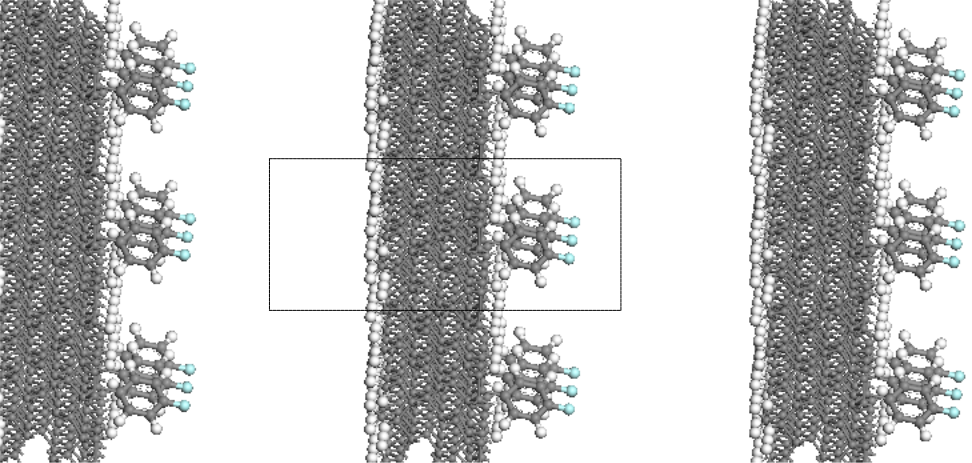
\includegraphics[width=.8\linewidth]{pictures/supercellvacuum.png}
\end{figure}

\printbibliography
\end{document}

